\documentclass[11pt]{article}

\usepackage[utf8]{inputenc}
\usepackage[margin=2cm]{geometry} 
\usepackage{hyperref}
\usepackage{graphicx}
\usepackage{float}
\usepackage{caption}
\usepackage{longtable}
\usepackage{minted}
\usepackage{appendix}
\usepackage{xcolor}
\usepackage{subfig}
\usepackage{bookmark}
\usepackage{array}
\usepackage{multirow}
\usepackage{rotating}

\setlength{\parskip}{1em}
\setlength{\parindent}{0pt}

\begin{document}

% ============ TITLE PAGE ============
\title{\huge Data Mining \& Machine Learning F20DL} 
% \\ {\small{\url{ }}}}
\author{Group 4\\Lewis Wilson, Sam Fay-Hunt, Kamil Szymczak, Chun Man }
\date{\today}
\maketitle

% ============ TABLE OF CONTENTS ============
\newpage
\tableofcontents
\thispagestyle{empty}
\pagebreak
\setcounter{page}{1}
% ============   ============   ============

\newpage
\section{Variation in performance with size of the training and testing sets}

\newpage
\section{Variation in performance with change in the learning paradigm (Decision Trees versus
Neural Nets)}

\newpage
\section{Variation in performance with varying learning parameters in Decision Trees}

\subsection{J48}



\newpage
\subsection{Random Forest}

"max\_features" has the options "auto", "sqrt" and "log2". From (Figure \ref{AccOverTimeRF}) we can see that "sqrt" has a higher accuracy overall, the accuracy of "log2" varies between the lower end and the median accuracy value.
\par
“min\_samples\_split” has very little impact on accuracy.
\par
“criterion” gives a perfect negative correlation with respect to accuracy. Correlation values -  [Gini = -0.404 ], [Entropy = 0.404 ].
\par
“n\_estimators” which defines the number of trees in the forest seems to have very little correlation but high importance.
\par
“min\_samples\_leaf” gives a strong negative correlation in terms of accuracy, meaning the higher minimum samples at a leaf node, the lower the accuracy.
\par
“min\_weight\_fraction\_leaf” has a somewhat positive correlation.



\newpage
\section{Variation in performance with varying learning parameters in Neural Networks}
\subsection{Linear Classifier}



\newpage
\subsection{Multilayer Perceptron}



\newpage
\section{Variation in performance according to different metrics (TP Rate, FP Rate, Precision,
Recall, F Measure, ROC Area)}

% ============ APPENDICES BEGINNING ============
\pagebreak
\appendix
\appendixpage
\addappheadtotoc
\begin{appendices}

\section{Appendix A}

% =================== Workload Split Table ===================

\subsection{Workload split}
  
  \begin{table}[ht]
    \centering
    \begin{tabular}{|p{0.2\linewidth} | p{0.8\linewidth}|} 
      \hline
      \textbf{Team member}  & \textbf{Involvement} \\ \hline
      Lewis Wilson & text here \\ \hline
      Chun Man & text here  \\ \hline
      Sam Fay-Hunt & text here \\ \hline
      Kamil Szymczak & text here \\ \hline
    \end{tabular}
  \end{table}\label{ContributionTab}

As a team we are happy with everyone's contributions to the project. All team members were punctual and showed up to all scheduled meetings. Sam took the lead as project manager throughout the project delegating the workload and providing support to others.






% =================== J48 here ===================



% =================== Random Forest here ===================

\newpage
\begin{sidewaysfigure}[h!]
    \caption {Accuracy over time - Random Forest} \label{AccOverTimeRF}
    \centering
    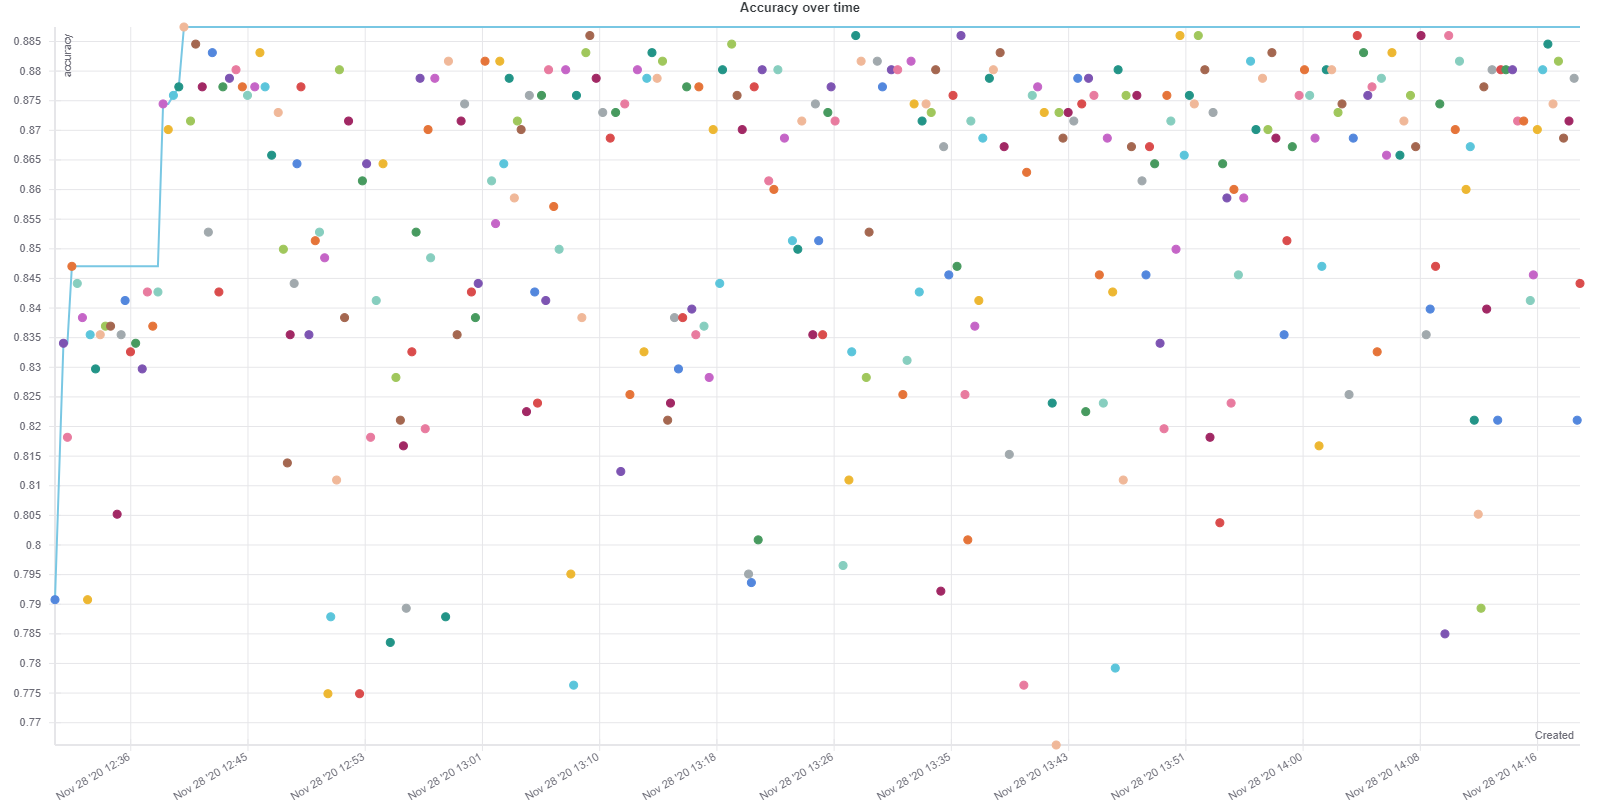
\includegraphics[width = \textwidth, height = \textwidth, keepaspectratio]{Images/RF Acc over time.png}
\end{sidewaysfigure}

\newpage
\begin{sidewaysfigure}[h!]
    \caption {Random Forest Parameters} \label{ParallelCoordRF}
    \centering
    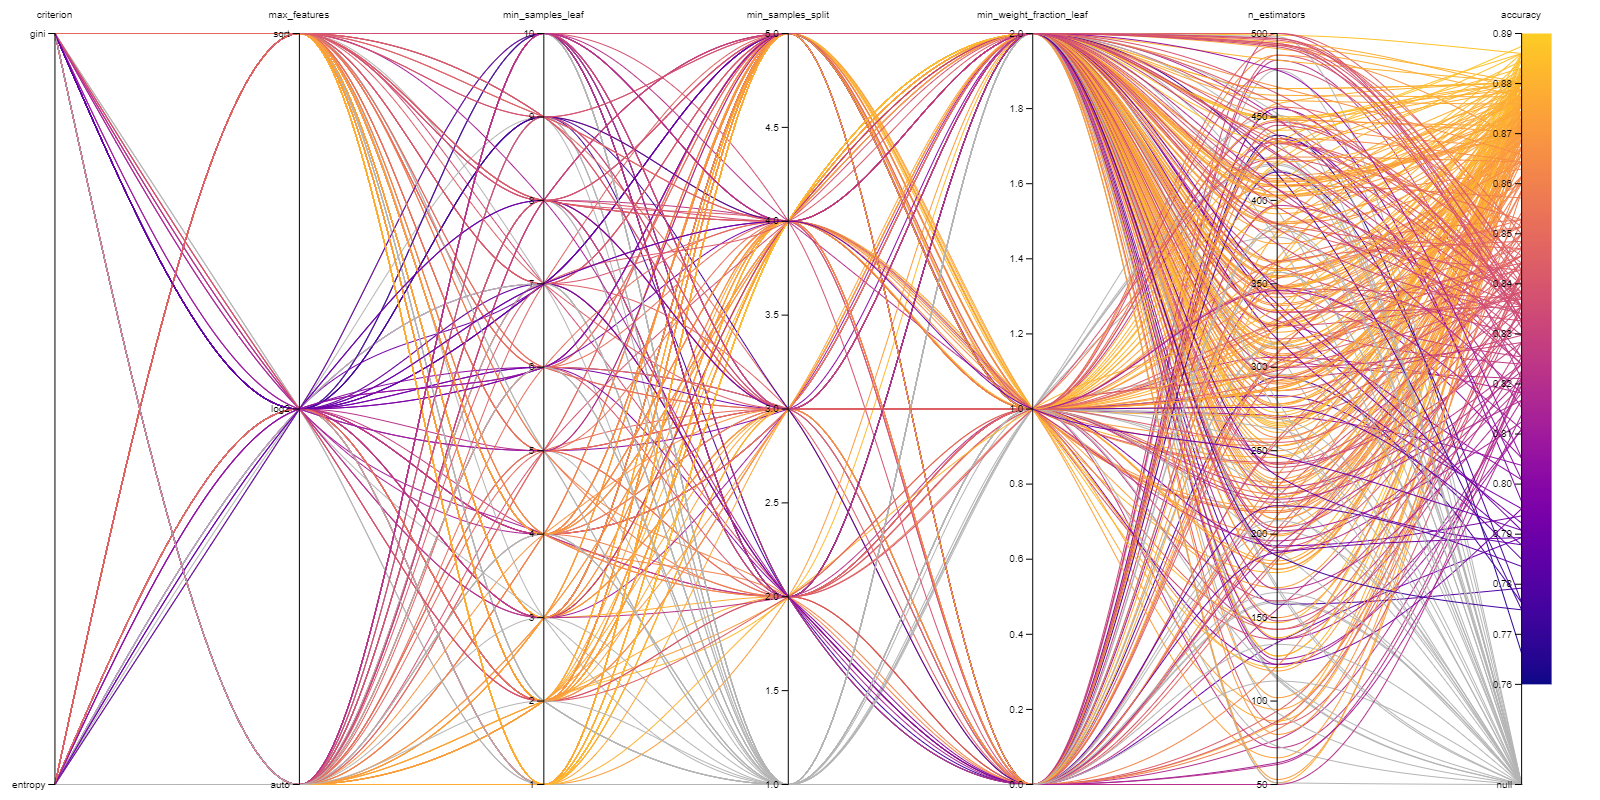
\includegraphics[width = \textwidth, height = \textwidth, keepaspectratio]{Images/RF ParallelCoordGraph.png}
\end{sidewaysfigure}

\subsection{Random Forest Parameter Importance}
  \begin{table}[ht]
    \centering
    \begin{tabular}{|p{0.3\linewidth} | p{0.3\linewidth}| p{0.3\linewidth}|} 
      \hline
      \textbf{Parameter Config}  & \textbf{Importance} & \textbf{Correlation} \\ \hline
        min\_samples\_split & 0.05 & 0.306 \\ \hline
        min\_samples\_leaf & 0.375 & -0.725 \\ \hline
        n\_estimators & 0.015 & 0.092 \\ \hline
        min\_weight\_fraction\_leaf & 0.014 & 0.123 \\ \hline
    \end{tabular}
  \end{table}\label{RF_ParamImp}

  \begin{table}[ht]
    \centering
    \begin{tabular}{|p{0.3\linewidth} | p{0.3\linewidth}| p{0.3\linewidth}|} 
      \hline
      \textbf{Parameter Config}  & \textbf{Importance} & \textbf{Correlation} \\ \hline
      max\_features.value\_sqrt & 0.010 & 0.563 \\ \hline
      max\_features.value\_log2 & 0.959 & -0.752 \\ \hline
      criterion.value\_entropy & 0.456 & 0.404 \\ \hline
      criterion.value\_gini & 0.544 & -0.404 \\ \hline
    \end{tabular}
  \end{table}\label{RF_ParamImp}
  
% =================== Linear Classifier here ===================



% =================== Multilayer Perceptron here ===================
\end{appendices}

\end{document}